\documentclass[../main.tex]{subfiles}

\begin{document}
Nuestro objetivo en este capítulo es presentar una definición de los lenguajes regulares mediante la Teoría de categorías, para los cuales existen tres maneras clásicas de definirlos:
\begin{enumerate}
    \item con una gramática generativa, cuya ventaja es producir fácilmente expresiones válidas para un lenguaje regular $\cal{L}$. Estas gramáticas también son conocidas como gramáticas de tipo 3 en la jerarquía de Chomsky;
    \item a través de expresiones regulares, usadas habitualmente para el reconocimientos de patrones simples; y
    \item por medio de autómatas finitos deterministas, el modelo de computo básico asociado a la validación de cadenas perteneciente a un lenguaje $\mathcal{L}$.
\end{enumerate}
Dado un lenguaje regular $\mathcal{L}$ definiremos una categoría cuyos objetos son las cadenas sobre un conjunto finito de símbolos, llamado el alfabeto, $\Sigma$ y sus morfismos corresponden a las reglas de producción en $\mathcal{L}$. Para esta tarea es necesario saber cómo generar una categoría a partir de una colección de funciones (generadores o, en este caso, reglas de producción) sobre un conjunto, así que iniciaremos definiendo las herramientas categóricas necesarias, proseguiremos con la definición de un lenguaje regular por medio de una categoría y mostraremos su equivalencia con las definiciones anteriores.  


\section{Categorías libres}
La noción de categoría libre es análoga a la de espacio vectorial generado por una base, es decir, dado un conjunto $X$ y un campo $k$, sabemos como construir un $k-$espacio vectorial $V$ que contenga a $X$. \\
En nuestro caso, los ingredientes de una categoría libre son un conjunto $G_0$, cuyos elementos serán los objetos en la categoría libre, y un conjunto $G_1$ de funciones en $G_0$ cuyos elementos serán los generadores de los morfismos; así, introducimos los siguientes conceptos que servirán como los cimientos de una categoría libre.  

\begin{dfn}
	Una \textbf{signatura simple} \(G\) es un conjunto de vértices \(G_0\) y un conjunto de aristas \(G_1\) tal que cada arista tiene asociado dos vértices, un dominio y un codominio
	$$\signature{G_1}{G_0}$$
    Notemos que una signatura simple induce una gráfica dirigida y viceversa, así que usaremos indistintamente ambos conceptos. \\
	Dadas \( G, \Gamma\) signaturas simples, un \textbf{homomorfismo de signaturas} \( \phi:G \to \Gamma\) es un par de funciones \( \phi_0: G_0 \to \Gamma_0\) y \( \phi_1: G_1 \to \Gamma_1\) tal que el siguiente diagrama conmuta, es decir, $\dom \circ \varphi_1 = \varphi_0 \circ \dom$ y $\cod \circ \varphi_1 = \varphi_0 \circ \cod$.  
	\[
	\begin{tikzcd}
		G_0 \arrow{d}{\phi_0} & G_1 \arrow{r}{\tt{dom}} \arrow{l}{\tt{cod}} \arrow{d}{\phi_1} & G_0 \arrow{d}{\phi_0} \\
		\Gamma_0 & \Gamma_1 \arrow{r}{\tt{dom}} \arrow{l}{\tt{cod}} & \Gamma_0
	\end{tikzcd}
	\]
\end{dfn}
\noindent Observemos que si consideramos dos homomorfismos de signaturas $\phi=(\phi_0, \phi_1): G \to \Gamma$ y $\psi =(\psi _0, \psi_1): \Gamma \to \Phi$ 
podemos tomar su composición entrada a entrada, es decir, $\psi \circ \phi = (\psi_0 \circ \phi_0,\psi_1 \circ \phi_1)$, la  cuál resulta nuevamente un homomorfismo de signaturas ya que el siguiente diagrama conmuta, pues, el rectángulo inferior y superior conmutan.

\[
\begin{tikzcd}
	G_0 \arrow{d}{\phi_0} & G_1 \arrow{r}{\tt{dom}} \arrow{l}{\tt{cod}} \arrow{d}{\phi_1} & G_1 \arrow{d}{\phi_0} \\
	\Gamma_0 \arrow{d}{\psi_0} & \Gamma_1 \arrow{r}{\tt{dom}} \arrow{l}{\tt{cod}} \arrow{d}{\psi_1} & \Gamma_1 \arrow{d}{\psi_0} \\
	\Phi_0 & \Phi_1 \arrow{r}{\tt{dom}} \arrow{l}{\tt{cod}} & \Phi_1 \\
\end{tikzcd} 
\]

\noindent Notemos, además, que la composición anterior es asociativa, pues lo es en cada entrada y que la identidad $Id_\Gamma=(Id_{\Gamma_0}, Id_{\Gamma_1})$ 
satisface que $Id_\Gamma \circ \phi = \phi$ y $\psi \circ Id_\Gamma = \psi$. Por lo anterior, tenemos una categoría cuyos objetos son las signaturas simples y sus flechas son los homomorfismos, la cual denotaremos $\bf{Sig}$ (en la literatura es usual denotarla $\bf{Graph}$).\\
Consideremos ahora la categoría \( \bf{Cat} \) cuyos objetos son categorías pequeñas, aquellas cuya colección de objetos es un conjunto, y las flechas son los funtores entre ellas. Definimos el funtor
\[
	U : \bf{Cat} \to \bf{Sig}
\]
tal que para cada categoría $\mathcal{C}$, $\bf{U}(\mathcal{C})$ es la gráfica dirigida cuyos vértices son los objetos $\mathcal{C}_0$, y las aristas corresponden a los morfismos, $\mathcal{C}_1$. Y, claramente, cada funtor $f: \cal{C} \to \cal{C'}$ induce un homomorfismo de gráficas $U (f): U(\cal{C}) \to U(\cal{C'})$. \\
Notemos que $U$ solamente olvida la operación de composición de morfismos en una categoría para obtener la gráfica subyacente, es por ello que  decimos que $U$ es un funtor olvidadizo. \\
Ahora, nuestro objetivo es definir un funtor $$F: \bf{Sig} \to \bf{Cat}$$
Dada una gráfica dirigida $G$, los objetos de $F(G)$ serán los vértices de $G$, y sus morfismos son de alguna de las siguientes dos formas:
\begin{itemize}
	\item Para cada $v$ vértice de $G$, tenemos un morfismo $\id_v: v \to v$; y
	\item para cualquier $n \in \mathbb{N}$ y para cualesquiera $e_1, ... , e_n$ aristas de $G$ tales que $\tt{cod} (e_i)=\tt{dom} (e_{i+1})$ con $i \in \{ 1, ..., n-1\}$ tenemos un morfismo $e_1 \dots e_n : \tt{dom} (e_1) \to \tt{cod} (e_n)$.
\end{itemize}
Es decir, los morfismos corresponden a las identidades y a todos los posibles caminos dirigidos dentro de la gráfica $G$. La composición de dos caminos está dada por la concatenación, salvo las identidades que se operan como la cadena vacía. Como la concatenación es siempre asociativa, concluimos que $F(G)$ es una categoría. \\
Ahora, tomemos $\phi: G \to G'$ un homomorfismo de gráficas; definimos el funtor $F(\phi): F(G) \to F(G')$ de la siguiente manera:   
\begin{itemize}
	\item Para cada $v$ objeto en $F (G)$, $(F(\phi))(v)=\phi_0(v) $;
	\item Para cada $I_v$ morfismo identidad de $F (G)$, $(F(\phi))(I_v)=I_{\phi_0(v)} $; y 
	\item Para cada $e_1 \dots e_n$ camino de $G$, $(\mathbf{F}\phi)(e_1 \dots e_n)=\phi(e_1) \dots \phi(e_n)$
\end{itemize}
Hacemos notar que el último inciso está bien definido pues $\phi$ es un homomorfismo de gráficas. A $F$ le llamamos \textbf{funtor libre}, en virtud de la siguiente proposición, pues dada una gráfica dirigida, $F$ construye la categoría libre asociada. 

\begin{prop}
	Sea $G$ una gráfica dirigida. Entonces existe un homomorfismo de gráficas $\eta:G \to UF(G)$ tal que para cualquier categoría $\cal{C}$ y un homomorfismo de gráficas $\phi: G \to U(\cal{C})$ existe un único funtor $\tilde\phi: F(G) \to \cal{C}$
	que hace conmutar el siguiente diagrama:
	
	\[
	\begin{tikzcd}
		F(G) \arrow[dashed]{d}{\tilde\phi}& G \arrow{r}{\eta} \arrow[swap]{rd}{\phi} & UF(G) \arrow[dashed]{d}{U(\tilde\phi)} \\
		\mathcal{C} & & U(\cal{C})
	\end{tikzcd}
	\] 	
\end{prop}

\noindent En otras palabras, nos dice que siempre que metamos una gráfica $G$ en una categoría $\mathcal{C}$ por medio de un homomorfismo de gráficas, podemos extenderlo a un funtor de $F(G)$ en $\mathcal{C}$.

\begin{proof}
    Sea $G$ una gráfica dirigida. Vamos a definir a $\eta:G \to UF(G)$, para ello observemos que $UF(G)$ es la gráfica cuyos vértices son los vértices de $G$ y hay un arista de $v$ a $w$ en $UF(G)$ cada que hay un camino de $v$ a $w$ en $G$. \\ 
	Definimos $\eta:G \to \mathbf{UF}G$ como $\eta_1$ la identidad en vértices y dado un arista $e:v_1 \to v_2$ en $G$, por el comentario anterior es un arista en $UF(G)$, definimos   $\eta_1(e)=e$. Así $\eta$ es la inclusión de $G$ en $UF(G)$ y, por lo tanto, un homomorfismo de gráficas. \\
    Sea $\cal{C}$ una categoría y $\varphi:G \to U(\cal{C})$ un homomorfismo de gráficas. Queremos definir un funtor $\tilde \phi : F(G) \to \cal{C}$.
    Sea $v$ un objeto de $F(G)$, entonces es un vértice $G$, así $\phi(c) \in U(\cal{C})$ y, por lo tanto, es un objeto en $\cal{C}$. Por lo tanto, $\tilde\phi (v) = \phi(v)$. \\
    Sea $f$ un morfismo de $F(G)$, tenemos los siguientes casos de acuerdo a la definición de morfismos en $F(G)$:
    \begin{itemize}
        \item Si $f=\id_v$ para algún $v$ vértice de $G$, entonces $\tilde\phi (\id_v) = \id_{\phi(v)}$
        \item Si $f=e: v \to w$, como $\phi$ es un homomorfismo de gráficas, entonces hay un arista $\phi_1(e): \phi_0(v) \to \phi_0(w)$ en $U(G)$ y, por lo tanto, hay un morfismo $\tilde\phi (e) :\tilde\phi(v) \to \tilde\phi(w)$ en $\cal{C}$. 
        \item Si $f=e_1 \dots e_n$, definimos $\tilde\phi(f)= \tilde\phi(e_n) \circ \cdots \circ \tilde\phi(e_1)$
    \end{itemize}
    De las condiciones anteriores se sigue inmediatamente que $\tilde \phi$ es funtor. Sigue ver que el diagrama conmuta, pero es claro puesto que $\eta$ y $U$ actúan como inclusiones tanto en vértices como en aristas. \\
\end{proof}

A continuación definiremos la clase de lenguajes generados por una signatura simple y posteriormente mostraremos que son exactamente los lenguajes regulares. \\
A partir de esta sección, dada una signatura simple denotaremos como $\mathcal{C}(G)$ a la categoría libre generada por $G$. 
Sea $V$ un conjunto no vacío de símbolos, llamado vocabulario, y $G$ una signatura simple. A cada arista de $G$ le asociaremos una palabra en $V$ mediante una función $L: G_1 \to V$, o equivalentemente, un homomorfismo de gráficas $L: G \to V$ donde $V$ es la gráfica con un vértice y cada palabra es una arista. Observemos que podemos extender $L$ de la siguiente forma: para cada morfismo $f=f_n \circ \dots \circ f_1$ en $\mathcal{C}(G)$, $L^*(f)=L(f_1)\cdots L(f_n) \in V^*$ y $L^*(Id_v)=\varepsilon$ para cualquier $v \in G_0$, donde $V^* $ denota a la estrella de Kleene de $V$, es decir, el conjunto de cadenas finitas con símbolos en $V$. \\

\begin{dfn}
	Una \textbf{gramática simple} es una signatura finita simple $G$ junto a un homomorfismo de gráficas $L: G \to V$  y símbolos distinguidos $s_0, s_1 \in G_0$, llamados el símbolo inicial y el terminal. Así, tenemos el siguiente diagrama:  
	
	\[
	\begin{tikzcd}
		G_0 & G_1 \arrow{l}{\texttt{dom}} \arrow{r}{\texttt{cod}} \arrow{d}{L} & G_0 \\
		& V &
	\end{tikzcd}
	\]
El \textbf{lenguaje generado por $G$} se define como: \\
	\[
		\mathcal{L}(G)=L^*(\mathcal{C}(G)(s_0,s_1)) \subset V*
	\]
Es decir, es la imagen bajo el funtor $L*$ de todos los morfismos en $\mathcal{C}$ con dominio el símbolo inicial y codominio el símbolo terminal.  \\
	Un \textbf{morfismo de gramáticas simples} $\phi : G \to H$ es un homomorfismo de gráficas tal que el siguiente diagrama conmuta
	\[
		\begin{tikzcd}
			G \arrow{rr}{\phi} \arrow[swap]{rd}{L_G} & & H \arrow{ld}{L_H} \\
			& V &
		\end{tikzcd}
	\]
	
\end{dfn}

\begin{ej}
    \label{AconoceB}
	Consideremos la siguiente gráfica $G$: 
	\begin{center}
	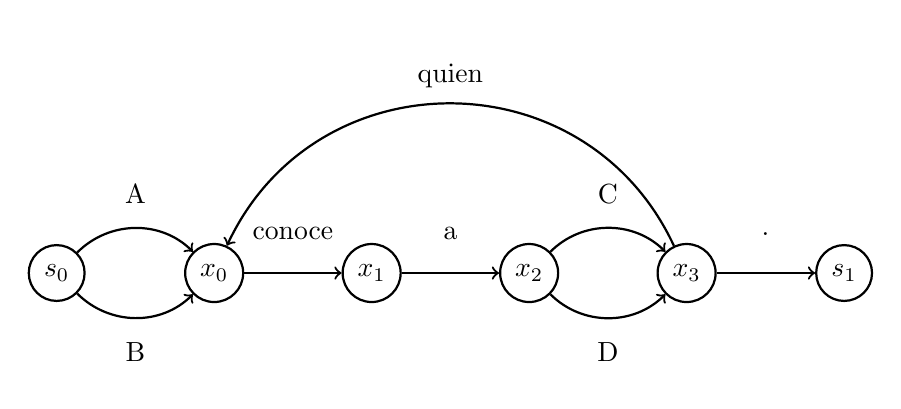
\begin{tikzpicture}[node distance={20mm}, thick, main/.style = {draw, circle},
	protein/.style={circle,draw=white,very thick}] 
		\node[main] (1) {$s_0$}; 
		\node[main] (2) [right of=1] {$x_0$}; 
		\node[main] (3) [right of=2] {$x_1$}; 
		\node[main] (4) [right of=3] {$x_2$}; 
		\node[main] (5) [right of=4] {$x_3$}; 
		\node[main] (6) [right of=5] {$s_1$}; 
		\node[protein] (p) at (1,1)  {A};
		\node[protein] (p) at (1,-1)  {B};
		\node[protein] (p) at (3,.5)  {conoce};
		\node[protein] (p) at (5,.5)  {a};
		\node[protein] (p) at (5,2.5)  {quien};
		\node[protein] (p) at (7,1)  {C};
		\node[protein] (p) at (7,-1)  {D};
		\node[protein] (p) at (9,.5)  {.};
		\draw[->] (2) -- (3);
		\draw[->] (3) -- (4);
		\draw[->] (5) -- (6);
		\draw[->] (1) to [out=45, in=135, looseness=1] (2); 
		\draw[->] (1) to [out=315, in=225, looseness=1] (2); 
		\draw[->] (5) to [out=115, in=65, looseness=1.2] (2);    
		\draw[->] (4) to [out=45, in=135, looseness=1] (5); 
		\draw[->] (4) to [out=315, in=225, looseness=1] (5); 
	\end{tikzpicture}
	\end{center}	
	Notemos que induce claramente una gramática simple. Algunos elementos de su lenguaje generado son ''A conoce a C'', ''B conoce a D quien conoce a C'' y ''A conoce a C quien conoce a D quien conoce a D''.    
\end{ej}
Es necesario preguntarse cuál es la clase de lenguajes que son producidos por medio de estas signaturas; afortunadamente, la respuesta es sencilla: 
 la clase de los lenguajes regulares. Para probar esta afirmación, introducimos la siguiente definición. 

 \begin{dfn}
 	
 	Una \textbf{gramática regular o de tipo 3} es una tupla $(N,V,P,s_0)$ donde $V$ es un vocabulario no vacío; $N$ es un conjunto de símbolos no terminales con un símbolo de inicio $s_0$; y $P$ un conjunto finito de reglas de producción, cada una de alguna de las siguientes formas:
 	
 	$$A \to aB$$
 	$$A \to a$$
 	$$A \to \epsilon$$
    con $A$ y $B$ en $N$, y $a \in V$. \\
    Diremos que \textbf{$\beta$ se deriva de $\alpha$} denotado $\alpha \Rightarrow \beta$ si y sólo si existen $\gamma, \theta, \kappa, \lambda$ tales que $\alpha = \gamma \kappa \theta$, $\beta = \gamma \lambda \theta$ y $\kappa \to \lambda$ es una regla de producción. Definimos $\Rightarrow^*$ como la cerradura transitiva\footnote{Sea $R\subset A \times A$ una relación. Definimos la cerradura transitiva de $R^*$ como $xR^*y$ si y sólo si hay $a_1,...,a_n \in A$ tales que $xRa_1,a_1R_2,...,a_{n-1}Ra_n$ y $a_nRy$.} de $\Rightarrow$. \\
 	Definimos el lenguaje $L$ generado por una gramática regular como 
    $$\mathcal{L} = \{ w \in V^*|s_0 \Rightarrow^*w \}$$
 	Decimos que un \textbf{lenguaje es regular} si es generado por un gramática regular.
 \end{dfn}
 
 \begin{ej}
 	Consideremos la siguiente gramática regular con los símbolos no terminales $N= \{A, s_0\}$, el vocabulario $V=\{a, b, c\}$ y con las siguientes reglas $P$:
 	\begin{align*}
		s_0 &\to as_0 \\
		s_0 &\to bA \\
		A &\to \epsilon \\
		A &\to cA
 	\end{align*} 
 	Observemos que el lenguaje generado por dicha gramática es $L=\{ a^i b c^j|i, j \in \mathbb{N} \}$  
 \end{ej}
 
 Con la definición anterior, ya estamos en condiciones para demostrar el teorema principal de este capítulo:
 
 
 \begin{thm}
	\begin{enumerate}[label=(\alph*)]
 		\item Todo lenguaje regular es generado por una gramática simple.
 		\item Todo lenguaje generado por una gramática simple es regular.
 \end{enumerate}	

 \end{thm}
 
 \begin{proof}
 	
 	
 	Primero probemos $(a)$.\\
 	Sea $L$ un lenguaje regular generado por la gramática $(N,V,P,s)$. \\
 	Definimos una gramática simple $G=P \rightrightarrows (V \cup \{ s, \epsilon \})$ donde para cada $p$ regla de producción:
 	\begin{itemize}
 		\item Si $p$ es de la forma $A \to aB$ con $A,B \in N$ y $a \in V$ entonces $p:A \to B$ en $G$ y $L(p)=a$.
 		\item Si $p$ es de la forma $A \to a$ con $A \in N$ y $a \in V$, entonces $p:A \to s_1$ en $G$ y $L(p)=a$
 		\item Si $p$ es de la forma $A \to \epsilon$ con $A \in N$, entonces $p:A \to s_1$ en $G$ y $L(p)=\epsilon$
 	\end{itemize}
    Observación. El símbolo $\epsilon$ de nuestro vocabulario cubrirá el papel de la cadena vacía. \\
 	
 	Probemos que $L=L(G)$.\\
 	Sea $w \in L$. 
 	Entonces existe una derivación
 	\[ s_0 \xRightarrow{p_1} \cdots \xRightarrow{p_n} w\]
 	Observemos que si $n=1$, entonces $p_1$ es de la forma $s \to w$, así tenemos el morfismo $p_1: s_0 \to s_1$ tal que $L(p_1)=w$.
 	Ahora, si $n>1$ veamos que la derivación es necesariamente de la forma: 
 	\[ s_0 \xrightarrow{p_1} aA_1 \xrightarrow{p_2} \cdots \xrightarrow{p_{n-1}} uA_{n-1} \xrightarrow{p_n} w\]
 	donde $A_i \in N$ con $i \in \{ 1, ..., n-1 \}$, $a\in V$ y $u \in V^*$. Así tenemos los siguientes morfismos en $G$: 
 	
 	\[ s_0 \xrightarrow{p_1} A_1 \xrightarrow{p_2} \cdots \xrightarrow{p_{n-1}} A_{n-1} \xrightarrow{p_n} s_1\]
 	
 	Entonces el morfismo $p =  p_n \circ p_{n-1} \circ \dots \circ p_2 \circ p_1: s_0 \to s_1$ y
 	\begin{align*}
	 	 L(p)=L(p_n \circ p_{n-1} \circ \dots \circ p_2 \circ p_1) &=(L(p_1) L(p_2) \dots L(p_n)) L(p_{n-1}) \\
	 	 &= u L(p_{n-1}) = w
 	\end{align*}
 	Observemos que es posible que $L(p_{n-1}) = \epsilon$ pero en ese caso $u = u \epsilon = w$. \\
 	Por lo tanto, $w \in L(G)$. Así, $L \subset L(G)$\\
 	Ahora, sea $w \in L(G)$. 
 	Entonces existe $f:s_0 \to s_1$ en $\mathcal{C}(G)$ tal que $L(f)=w$. Como $\mathcal{C}(G)$ es una categoría libre, entonces $f$ es un camino en $G$, así existen $p_1, \dots, p_n$ reglas de producción en $P$ tal que $f=p_n \circ ... \circ p_1$ que inducen una derivación: 
 	\[
 		s_0 \xRightarrow{p_1} \cdots \xRightarrow{p_n} w
 	\]
 	Y, por lo tanto, $w \in L$. Así $L(G) \subset L$. \\
 	Con ello concluimos que $L=L(G)$ y terminamos la prueba del inciso (a). \\
    
 	Vayamos con la prueba de (b) \\
 	Sea $G$ una gramática simple con el homomorfismo $L: G \to V$ con $V$ vocabulario. \\
    La estrategia será construir un autómata finito no determinista (AFND) que admite el lenguaje $L(G)$, lo cual implica que $L(G)$ es un lenguaje regular, cuya prueba se puede consultar en \cite{hopcroft01}. \\
 	Definimos el AFND $M$ de la siguiente manera: su conjunto de estados es $G_1$, es decir, los vértices de $G$, donde $s_0$ es el símbolo de inicio y $F=\{s_1\}$ el conjunto de estados finales, y tomemos $V$ como el conjunto de entradas. Definimos la función de transición $\delta : G_0 \times V \to 2^{G_0}$ tal que para cada $q \in G_0$ y $v\in V$, 
 	\[
 		\delta (q,v) = \{q'|\exists f: q \to q' \in G_1 \text{ tal que }L(f)=v \}
 	\]
 	Recordemos que $\delta$ se extiende recursivamente a $V^*$ de la siguiente manera:
 	\begin{align*}
 		&\delta ^* (q, \epsilon) = \{ q \} \\
 		&\delta ^* (q, xa) = \bigcup_{r \in \delta ^* (q,a)} \delta (r,a)
 	\end{align*}
	Así, definimos el lenguaje aceptado por $M$ como:
	\[
		L(M)=\{x \in V^* | \delta ^* (s_0, x) \cap {s_1} \neq \varnothing \}
	\]
 	Probemos que $L(G)=L(M)$. \\
 	Sea $w \in L(G)$. Entonces existe $f:s_0 \to s_1$ en $\mathbf{C}(G)$ tal que $L(f)=q$. Observemos que entonces existen $f_1, \dots, f_n$ en $G_1$ tales que el siguiente diagrama conmuta: 
 	\begin{center}
 	\begin{tikzcd}
 		a_0=s_0 \arrow{r}{f_1} \arrow[rrrr,bend right, swap]{f} & a_ 1 \arrow{r}{f_2} & ... \arrow{r}{f_{n-1}} & a_{n-1} \arrow{r}{f_n} & s_1=a_{n+1}
 	\end{tikzcd}
	\end{center}
 	Así $q=L(f)=L(f_1) \cdots L(f_n)$, entonces observemos que para cada $i\in \{0, ..., n\}$, $a_{i+1} \in \delta (a_i, L(f_i))$ y, por lo tanto, $s_1=a_{n+1} \in \delta ^*  (a_0, L(f))=\delta ^*  (s_1, w)$. Como $\{s_1\}$ es el conjunto terminal, concluimos que $w \in L(M)$.  Por lo tanto, $L(G) \subset L(M)$. \\
 	Sea $w \in L(M)$ \\
 	Entonces $s_1 \in \delta ^* (s_0, w)$. \\
 	Observemos que si $w= \epsilon$, entonces $s_1 \in \delta (s_0, \epsilon)$, así hay un morfismo $f:s_0 \to s_1$ tal que $L^*(f)= \epsilon$, por la definición de $L^*$ esto implica que $f=Id_{s_0}$, así $s_0=s_1$ y $w \in L(G)$. \\ 
 	Por otro lado, si $w$ no es la cadena vacía, entonces hay $w_1,\dots, w_n \in V$ tales que $w=w_1 \cdots w_n$ y estados $q_1, \dots, q_{n-1}$ que satisfacen:
 	\begin{multicols}{3}
 		$q_1 \in \delta (s_0,w_1)$ \\
 		$q_{i+1} \in \delta (q_i,w_i)$ \\
 		$s_0 \in \delta (q_{n-1},w_n)$
 	\end{multicols} 
 	para $i \in \{ 1, ..., n-2 \}$. Esto significa que hay $f_1, \dots , f_n$ en $G_1$ tales que
 	
 	 \begin{center}
 		\begin{tikzcd}
 			s_0 \arrow{r}{f_1}  & q_ 1 \arrow{r}{f_2} & ... \arrow{r}{f_{n-1}} & q_{n-1} \arrow{r}{f_n} & s_1
 		\end{tikzcd}
 	\end{center}
 	y $L(f_i)=w_i$ con $i \in \{1, \dots n\}$. Por lo tanto, $f_n \circ ... \circ f_1 : s_0 \to s_1 \in \mathbf{C}(G)$ y 
 	\[
 		L^*(f_n \circ ... \circ f_1) = L(f_1) \cdots L(f_n)=w_1 \cdots w_n = w
 	\]
 	Por lo tanto, $w \in L(G)$ y así $L(M) \subset L(G)$. \\
 	Por ello, $L(G)=L(M)$ como queríamos demostrar. 
 \end{proof}
 
 A partir de ahora dejaremos de usar el término gramáticas simples y, en virtud del teorema anterior, las llamaremos gramáticas regulares. Denotaremos como $\mathbf{Reg_V}$ a la categoría cuyos objetos son gramáticas regulares y los morfismos son los homomorfismos entre ellas. \\
 Para ilustrar las pruebas anteriores, veamos los siguientes ejemplos:
 
 \begin{ej}
 	Consideremos la gramática regular del segundo ejemplo, observemos que su lenguaje es generado por la gramática de la siguiente gráfica:
 	
	\begin{center}
	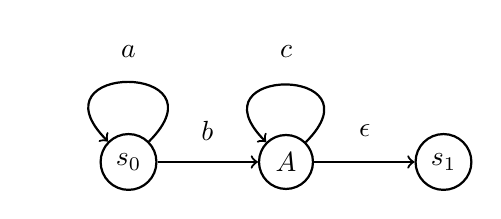
\begin{tikzpicture}[node distance={20mm}, thick, main/.style = {draw, circle},
		protein/.style={circle,draw=white,very thick}] 
		\node[main] (1) {$s_0$}; 
		\node[main] (2) [right of=1] {$A$}; 
		\node[main] (3) [right of=2] {$s_1$};
		\draw[->] (1) -- (2);
		\draw[->] (2) -- (3); 
		\draw[->] (1) to [out=45, in=135, looseness=7] (1);
		\draw[->] (2) to [out=45, in=135, looseness=7] (2);
		\node[protein] (p) at (0,1.4)  {$a$};
		\node[protein] (p) at (2,1.4)  {$c$};
		\node[protein] (p) at (1,.4)  {$b$};
		\node[protein] (p) at (3,.4)  {$\epsilon$};
	\end{tikzpicture}
	\end{center}
	Vale la pena notar que esta gráfica induce inmediatamente un autómata finito con épsilon transiciones\footnote{Una autómata fínito con epsilon transiciones es un autómata finito no determinista donde es posible transitir entre estados sin consumir símbolos. Esta modificación no aumenta, ni disminuye el poder expresivo del autómata. }. 
 \end{ej}
 	
 \begin{ej}
	 Consideremos la gramática regular del primer ejemplo, es claro que induce el siguiente AFND:
	 \begin{center}
	 	\begin{tikzpicture}[node distance={20mm}, thick, main/.style = {draw, circle},
	 		protein/.style={circle,draw=white,very thick}] 
	 		\node[main] (1) {$s_0$}; 
	 		\node[main] (2) [right of=1] {$x_0$}; 
	 		\node[main] (3) [right of=2] {$x_1$}; 
	 		\node[main] (4) [right of=3] {$x_2$}; 
	 		\node[main] (5) [right of=4] {$x_3$}; 
	 		\node[state, accepting] (6) [right of=5] {$s_1$}; 
	 		\node[protein] (7) [left of=1] {$start$};
	 		\node[protein] (p) at (1,1)  {A};
	 		\node[protein] (p) at (1,-1)  {B};
	 		\node[protein] (p) at (3,.5)  {conoce};
	 		\node[protein] (p) at (5,.5)  {a};
	 		\node[protein] (p) at (5,2.5)  {quien};
	 		\node[protein] (p) at (7,1)  {C};
	 		\node[protein] (p) at (7,-1)  {D};
	 		\node[protein] (p) at (9,.5)  {.};
	 		\draw[->] (7) -- (1);
	 		\draw[->] (2) -- (3);
	 		\draw[->] (3) -- (4);
	 		\draw[->] (5) -- (6);
	 		\draw[->] (1) to [out=45, in=135, looseness=1] (2); 
	 		\draw[->] (1) to [out=315, in=225, looseness=1] (2); 
	 		\draw[->] (5) to [out=115, in=65, looseness=1.2] (2);    
	 		\draw[->] (4) to [out=45, in=135, looseness=1] (5); 
	 		\draw[->] (4) to [out=315, in=225, looseness=1] (5); 
	 	\end{tikzpicture}
	 \end{center}
 \end{ej}

 Un resultado bien conocido sobre lenguajes regulares es que son cerrados respecto a uniones e intersecciones finitas. Existen diversas pruebas dependiendo de la definición preferida; mostremos entonces una en términos categóricos.  
 
 \begin{prop}
 	Los lenguajes regulares son cerrados bajo intersecciones y uniones finitas. 
 \end{prop}

 \begin{proof}
   	Sean $G$ y $G'$ gramáticas regulares con símbolos iniciales $s_0$, $s'_0$ y símbolos finales $s_1$, $s'_1$ respectivamente. \\
	Definimos la siguiente gramática regular $G \cap G': H_0 \subset G_1 \times G'_1 \rightrightarrows H_1 \subset G_0 \times G'_0$ de la siguiente forma: $(q_0,q'_0)$ y $(q_1,q'_1)$ son el símbolo inicial y final respectivamente. Además, existe un arista entre $(a,b)$ y  $(a',b')$ en $G \cap G'$ si y sólo si existen $a \xrightarrow{f} b$ en $G$ y $a' \xrightarrow{f'} b'$ en $G'$ tales que $L_G(f)=L_{G'}(f')$, denotaremos a dicho arista como $(f,f')$ y con ello definimos $L((f,f'))=L_G(f)$. \\
	Afirmación. $L(G \cap G') = L(G) \cap L(G')$. \\
	Tenemos que $w \in L(G \cap G')$ si y sólo si existe $(f,f'):(s_0,s'_0) \to (s_1, s'_1) \in \mathbf{C}(G\cap G')$ tal que $L^*(f,f')=w$, si y sólo existen $(f_1,f'_1), \cdots (f_n,f'_n)$ aristas de $G \cap G_1$ tales que el siguiente diagrama conmuta
	
	 \begin{center}
		\begin{tikzcd}
			(s_0,s'_0) \arrow{r}{(f_1.f'_1)} \arrow[rr,bend right, swap]{(f,f')} & ...  \arrow{r}{(f_n,f'_n)} & (s_1,s'_1)
		\end{tikzcd}
	\end{center}
 	y $w=L(f_1,f'_1) \cdots L(f_n,f'_n)$, pero esto ocurre si y sólo existen $f_1, ..., f_n$ aristas en $G$ y $f'_1, ..., f'_n$ aristas en $G'$ tales que los siguientes diagramas conmutan: 
 	\begin{multicols}{2}
 		 \begin{center}
 		\begin{tikzcd}
 				s_0 \arrow{r}{f_1} \arrow[rr,bend right, swap]{f} & ...  \arrow{r}{f_n} & s_1
 			\end{tikzcd}
 		\end{center}
 		
 		\begin{center}
 			\begin{tikzcd}
 				s'_0 \arrow{r}{f'_1} \arrow[rr,bend right, swap]{f'} & ...  \arrow{r}{f'_n} & s'_1
 			\end{tikzcd}
 		\end{center}
 	\end{multicols}
    \noindent y $w=L(f_1)\cdots L(f_1)=L(f'_1)\cdots L(f'_n)$, lo cual sucede si y sólo existen $f:s_0 \to s_1$ en $\mathbf{C}(G)$ y $f': s'_0 \to s'_1$ en $\mathbf{C}(G')$ tales que $L^*(f)=w=L^*(f')$. \\
    Lo anterior sucede si y sólo si $w \in L(G)$ y $w \in L(G')$. Por lo tanto $L(G\cap G')=L(G) \cap L(G')$. \\
 	Ahora, para probar el resultado en el caso de la unión definimos la gramática regular $G \cup G':G_0+G'_0 \rightrightarrows G_1+G_1'$ donde el símbolo $+$ representa la unión disjunta y además haremos la identificación $s_0=s'_0$ y $s_1=s'_1$. \\
 	Afirmación. $L(G \cup G') = L(G) \cup L(G')$. \\
 	Notemos que $w \in L(G \cup G')$ si y sólo si existe $f:s_0 \to s_1$ en $\mathbf{C}(G \cup G')$ tal que $L^*(f)=w$. \\
 	Procediendo de manera análoga a la prueba anterior, veremos que esto ocurre si y sólo si existe $f:s_0 \to s_1$ en $\mathbf{C}(G)$ o $f:s'_0 \to s'_1$ en $\mathbf{C}(G')$ tal que $L^*(f)=w$, pero esto se da cuando $w$ está en $L(G)$ o en $L(G')$. \\
 	Por lo tanto, $L(G\cup G') = L(G)\cup L(G')$. \\
 	Entonces, $L(G)\cap L(G')$ y $L(G)\cup L(G')$ son lenguajes regulares y procediendo inductivamente tenemos el resultado para uniones e intersecciones finitas. 
 \end{proof}
 
 Observemos que otra forma de interpretar lo anterior, es que dado dos objetos $G,G'$ en $\mathbf{Reg_V}$ encontramos dos objetos $G\cap G'$ y $G\cup G'$ en $\mathbf{Reg_V}$. La siguiente proposición nos dirá la manera en que se relacionan en la categoría. 
 
 \begin{prop}
	$\mathbf{Reg_V}$ tiene productos y coproductos finitos. Más aún, si $G, G'$ son objetos de $\mathbf{Reg_V}$, entonces $G\cap G'$ y $G\cup G'$ son su producto y coproducto respectivamente. 
 \end{prop}
 \begin{proof}
 	Sean $G$ y $G'$ en $\mathbf{Reg_V}$. \\
 	Primero veamos que $G\cap G'$ es el producto. \\
 	Sea $H$ en $\mathbf{Reg_V}$ junto con $f:H \to G$ y $g:H \to G'$ morfismos de gramáticas regulares. \\
 	Vamos a definir el morfismo de gramáticas regulares $(f,g):H \to G\cap G'$ de la siguiente manera:
 	\begin{itemize}
		\item Para cada vértice $v \in H_0$, $(f,g)_0(v)=(f_0(v),g_0(v))$, y
		\item para arista $h\in H_0$, $(f,g)_1(h)=(f_1(h),g_1(h))$
 	\end{itemize}
 	Veamos que es un morfismo de gramáticas regulares. Sea $h:v_1 \to v_2$ un arista de $H$. Como $f,g$ son morfismos de gramáticas regulares, entonces $f(h): f(v_1)\to f(v_2)$ y $g(h): g(v_1)\to g(v_2)$ son aristas $G$ y $G'$ respectivamente y, además, $L_G(f(h))=L_H(h)=L_{G'}(g(h))$ pues el siguiente diagrama conmuta: 
 	
 	\[
 	\begin{tikzcd}
 		G \arrow[swap]{rd}{L_G} & H \arrow{r}{g'} \arrow[swap]{l}{g} \arrow{d}{L_H}  & G' \arrow{ld}{L_{G'}} \\
 		& V 
 	\end{tikzcd}
 	\]
 	Así $(f,g)(h):(f,g)(v_1) \to (f,g)(v_2)$ está en $G_1 \cap G_2$ y $L_H(h)=L_{G\cap G'}((f,g)(h))$ como queríamos ver. \\
 	Ahora, vamos a definir las proyecciones $\pi : G\cap G' \to G$ y $\pi' : G\cap G' \to G'$ como las inducidas por las proyecciones $G \times G' \to G$ y $G \times G' \to G$, así como definimos $(f,g)$ entrada a entrada, tenemos que el siguiente diagrama conmuta: 
 	 \[
 	\begin{tikzcd} 		
 		& H \arrow{d}{(f,g)} \arrow[swap]{ld}{f} \arrow{rd}{g} & \\
 		G  & G\cap G' \arrow{l}{\pi} \arrow{r}{\pi'} & G'
 	\end{tikzcd}
 	\]
 	Supongamos entonces que existe un morfismo de gramáticas regulares $k: H \to G\cap G'$ tal que el siguiente diagrama también conmuta: 
 	 \[
	\begin{tikzcd} 		
		& H \arrow{d}{k} \arrow[swap]{ld}{f} \arrow{rd}{g} & \\
		G  & G\cap G' \arrow{l}{\pi} \arrow{r}{\pi'} & G'
	\end{tikzcd}
	\]
	Observemos que como $\pi$ y $\pi'$ las tomamos como las inducidas por las proyecciones del producto en aristas y vértices, entonces por unicidad en $\mathbf{Set}$ tenemos que $k_0=(f,g)_0$ y $k_1=(f,g)_1$ y, por lo tanto, $k=(f,g)$. \\
	Concluimos entonces que $G \cap G'$ es el producto de $G$ y $G'$ en $\mathbf{Reg_V}$ pues se satisface la propiedad universal. \\
	Probemos ahora que $G\cup G'$ es el coproducto. \\
	Sea $H$ en $\mathbf{Reg_V}$ junto con $f:G \to H$ y $g:G' \to H$ morfismos de gramáticas regulares. Definimos $[f,g]:G\cup G' \to H$ tal que para cada $v \in (G\cup G')_0$ y $h \in (G\cup G')$ como
	\begin{multicols}{2}
		\begin{equation*}
			[f,g]_0(v)=
			\begin{cases}
				f_0(v) & \text{if } v \in G_0\\
				g_0(v) & \text{if } v \in G'_0
			\end{cases}
		\end{equation*}
        
		\begin{equation*}
			[f,g]_1(h)=
			\begin{cases}
				f_1(h) & \text{if } h \in G_1\\
				g_1(h) & \text{if } h \in G'_1
			\end{cases}
		\end{equation*}
	\end{multicols}
	Puesto que $f,g$ son morfismos de gramáticas, el siguiente diagrama conmuta:
	
 	\[
	\begin{tikzcd}
		G \arrow{r}{g} \arrow[swap]{rd}{L_G} & H \arrow{d}{L_H}  & G' \arrow{ld}{L_{G'}} \arrow{l}{g'} \\
		& V 
	\end{tikzcd}
	\]
	Por la cual tenemos que $L_G(f(h))=L_H(h)=L_{G'}(g(h))$, y como $[f,g](h)=f(h)$ o $[f,g](h)=g(h)$, entonces $[f,g]$ es un morfismo de gramáticas regulares. \\
	Luego, definimos las inyecciones $i:G \to G \cup G'$ y $i':G' \to G \cup G'$ como las inclusiones, es decir, $i(g)=g$ y $i'(g')=g'$ para $g \in G$ y $g' \in G'$. Es entonces claro que el siguiente diagrama conmuta: 
	
 	 \[
	\begin{tikzcd} 		
		& H  & \\
		G \arrow[swap]{r}{i} \arrow{ru}{f} & G\cap G' \arrow{u}{[f,g]} & G' \arrow{l}{i'} \arrow[swap]{lu}{g}
	\end{tikzcd}
	\]
	
	Además, dado cualquier morfismo $k: G \cup G' \to H$ tal que el siguiente diagrama conmuta
	
	 	 \[
	\begin{tikzcd} 		
		& H  & \\
		G \arrow[swap]{r}{i} \arrow{ru}{f} & G\cap G' \arrow{u}{k} & G' \arrow{l}{i'} \arrow[swap]{lu}{g}
	\end{tikzcd}
	\]
	Entonces para cualesquiera vértice $v$ y arista $h$ en $G$ tenemos que 
	$k_0(v)=k_0\circ i(v) = f_0(v)$ y $k_1(h)=k_1\circ i(h) = f_1(h)$, en cambio si están en $G'$ obtenemos que $k_0(v)=k_0\circ i'(v) = g_0(v)$ y $k_1(h)=k_1\circ i'(h) = g_1(h)$. Por lo tanto, $[f,h]=k$ como queríamos probar. \\
	Por lo tanto, $G \cup G'$ es el coproducto de $G$ y $G'$. 
 \end{proof}

	
 
\end{document}
